\documentclass[fleqn]{MJD}

\usepackage{cancel}
\usepackage{cleveref}
\usepackage{titlesec}
\usepackage{hyperref}
%\colorsections
%\bluelinks
\newcommand{\problem}[1]{\chapter{Problem #1}}
\newcommand{\subproblem}[2]{\section{(#1)~ #2}}
\newcommand{\subsubproblem}[2]{\subsection{ #1)~ #2}}
\newcommand{\U}{\cup}
\renewcommand{\S}{\mathcal{S}}
\renewcommand{\s}{\subset}
\renewcommand{\equiv}{\Leftrightarrow}
\newcommand{\0}{\emptyset}
\newcommand{\imp}{\Rightarrow}
\newcommand{\Usum}{\bigcup\limits_{i=1}^\infty}
\newcommand{\intsum}{\bigcup\limits_{i=1}^\infty}
\newcommand{\infsum}{\sum\limits_{i=1}^\infty}
\newcommand{\sets}{\{A_1, A_2 \dots\} }
\newcommand{\nsets}{\{A_1, \dots, A_n \} }

\titleformat{\chapter}[display]
  {\normalfont\bfseries}{}{0pt}{\LARGE}
  
\graphicspath{ {../} }

%%%%%%%%%%%%%%%%%%%%%%%%%%%%%%%%%%%%
\begin{document}
\lstset{language=Python}

\titleAT[CS 224N: Assignment 1]{Peter Li}

%-------------------------------------
\problem{1: Softmax (10 pts)}
%-------------------------------------

%----------------------
\subproblem{a}{Softmax Invariance to Constant (5 pts)}
\noindent\textbf{Answer:} \\
\begin{equation}
\forall{i}, \nonumber
\end{equation}
\begin{align}
	(softmax(x + c))_{i} &= \frac{e^{(x_{i} + c)}}{\sum_{j} e^{(x_{j} + c)}} %
	 					= \frac{e^{x_{i}} \times e^{c}}{e^{c} \times \sum_{j} e^{x_{j}}} \nonumber \\
	%
					   &= \frac{e^{x_{i}} }{\sum_{j} e^{x_{j}}} %
					    = softmax(x)_{i} \nonumber
\end{align}
\textit{so, }\\
\begin{align}
softmax(x) = softmax(x + c) \nonumber
\end{align}

\vskip5em

%----------------------
\subproblem{b}{Softmax Coding (5 pts)}
\noindent \textbf{Answer:} \\

\noindent See code: $\sim$\verb|/q1_softmax.py|.

%-------------------------------------
\problem{2: Neural Network Basics (30 pts)}
%-------------------------------------

%----------------------
\subproblem{a}{Sigmoid Gradient (3 pts)}

\noindent \textbf{Answer:}

\begin{align}
	%
	\frac{d\sigma(x)}{dx}  &= \frac{d}{dx}(\frac{1}{1 + e^{-x}}) \nonumber \\
	%
	&= -\frac{1}{(1+e^{-x})^2}\frac{d}{dx}(1+e^{-x})=\frac{-1}{(1+e^{-x})^{2}}\frac{d}{dx}e^{-x}=\frac{-1}{(1+e^{-x})^{2}}\frac{-1}{(e^{x})^{2}}\frac{d}{dx}e^{x} \nonumber \\
	%
	&=\frac{-1}{(1+e^{-x})^2}\frac{-1}{(e^{x})^{2}}e^{x}=\frac{1}{(1+e^{-x})^{2}(e^{x})^{2}}e^{x} \nonumber \\
	%
	&= \frac{e^{-x}}{(1+e^{-x})^2} =\frac{1+e^{-x}-1}{(1+e^{-x})^2} = \frac{1}{1+e^{-x}}-\frac{1}{(1+e^{-x})^{2}}\nonumber \\
	%
	&=(\frac{1}{1+e^{-x}})(1-\frac{1}{1+e^{-x}}) \nonumber \\
	%
	&= \sigma(x) (1 - \sigma(x)) \nonumber 
\end{align}


%----------------------
\newpage
\subproblem{b}{Softmax Gradient w/ Cross Entropy Loss (3 pts)}
\label{prob:2b}
\noindent \textbf{Answer:} 
\begin{equation}
	CE(\mathbf{y},\hat{\mathbf{y}}) = - \sum_{i} y_{i} log(\hat{y_{i}}) \nonumber
\end{equation}
\textit{ As $\mathbf{y}$ is one-hot vector, assume $y_{k}=1$, then other $y_{i}=0, \forall i\neq{k}$}

\begin{align}
	CE(\mathbf{y},\hat{\mathbf{y}}) = - y_{k}log(\hat{y}_{k}) = - log(\hat{y}_{k}) \nonumber
\end{align}
\textit {As, $\hat{y}_{k}=softmax(\bm{\theta})=\frac{e^{\theta_{k}}}{\sum_{j}{e^{\theta_{j}}}}$}
\begin{align}
	CE(\bm{\theta}) = - log(\frac{e^{\theta_{k}}}{\sum_{j}{e^{\theta_{j}}}}) \nonumber \\
	%
	=-\theta_{k} + log(\sum_{j}{e^{\theta j}}) \nonumber
\end{align}
\textit {So, for $y_{k}=1$}

\begin{align}
	\frac{\partial CE(\bm{\theta})}{\partial \bm{\theta}} = \frac{\partial}{\partial \bm{\theta}}(-\theta_{k} + log(\sum_{j}{e^{\theta_{j}}}) \nonumber \\
	= -\frac{\partial \theta_{k}}{\partial \bm{\theta}} + \frac{\partial}{\partial \bm{\theta}} log(\sum_{j}{e^{\theta_{j}}})
\end{align}
\textit {And,}
\begin{align}
	\frac{\partial \theta_{k}}{\partial \theta_{i}} &= %
\left\{
			\begin{array}{ll}
				 1 &, \mbox{if } i = k \\ 
				 0 &, \mbox{if } i \neq k
			\end{array}
		\right. \nonumber 
\end{align}
\textit {So, }
\begin{equation}
\frac{\partial \theta_{k}}{\partial \bm{\theta}}=\mathbf{y}
\end{equation}
\textit {And, }
\begin{align}
	\frac{\partial}{\partial \theta_{i}} log(\sum_{j}{e^{\theta_{j}}}) &= \frac{1}{\sum_{j}{e^{\theta_{j}}}}\frac{\partial}{\partial \theta_{i}}(\sum_{j}{e^{\theta_{j}}}) \nonumber \\
	%
	&= \frac{1}{\sum_{j}{e^{\theta_{j}}}}\frac{\partial}{\partial \theta_{i}}e^{\theta_{i}} \nonumber \\
	%
	&= \frac{e^{\theta_{i}}}{\sum_{j}{e^{\theta_{j}}}} \nonumber \\
	%
	&= softmax(\theta_{i})
\end{align}
\textit {With above equations,}
\begin{align}
	\frac{\partial CE(\bm{\theta})}{\partial \bm{\theta}} = -\mathbf{y} + \hat{\mathbf{y}} \nonumber
\end{align}
\vskip2em

\newpage

\subproblem{c}{One Hidden Layer Gradient (6 pts)}

\noindent \textbf{Answer:} \\
\\
\noindent \textit{To caculate $\frac{\partial J}{\partial x}$, where $J= CE(\mathbf{y}, \hat{\mathbf{y}})$ } \\
\\
\noindent Let $\bm{\theta}=\bm{hW}_{2} + \bm{b}_{2}$, and $\bm{Z1}=\bm{xW}_{1} + \bm{b}_{1}$ \\
\\
\noindent \textit{and from 2(b), we know $\frac{\partial}{\partial \bm{\theta}}CE(\mathbf{y}, \hat{\mathbf{y}})= -  \bm{y} + \bm{\hat{y}}$} \\
\\
\noindent \textit{we get, }
\begin{align}
	\frac{\partial J}{\partial \bm{\theta}} %
		&= \bm{\delta}_{3} = \hat{\bm{y}} - \bm{y} \nonumber \\
	%
	\frac{\partial J}{\partial \bm{h}} %
		&= \bm{\delta}_{2} = \bm{\delta}_{3} \frac{\partial \bm{\theta}}{\partial \bm{h}}= \bm{\delta}_{3}\bm{W}_{2}^{T} \nonumber \\
	%
	\frac{\partial J}{\partial \bm{Z1}} %
			&= \bm{\delta}_{1} = \frac{\partial J}{\partial \bm{h}} \frac{\partial \bm{h}}{\partial \bm{Z1}} = \bm{\delta}_{2} \circ \sigma'(\bm{Z1}) \nonumber \\
	%
	\frac{\partial J}{\partial \bm{x}} %
		&= \bm{\delta}_{1} \frac{\partial \bm{Z1}}{\partial \bm{x}} \nonumber \\
	%
		&= \bm{\delta}_{1}  \bm{W}_{1}^{T} \nonumber
\end{align}

%----------------------
\subproblem{d}{No. Parameters (2 pts)}

\noindent \textbf{Answer:} \\
\\
\textit {$\bm{W_{1}}$,$\bm{W_{2}}$,$b_{1},b_{2}$ are parameters. And $\bm{W1} \in \mathbb{R}^{D_{x} \times H}$, $\bm{W2} \in \mathbb{R}^{H \times D_{y}}$, $b_{1} \in \mathbb{R}^{H}$, $b_{2} \in \mathbb{R}^{D_{y}}$} \\
\\
\textit {In total, parameter count is}
\begin{align}
	(D_{x} \times H) + H + (H \times D_{y}) + D_{y} \nonumber
\end{align}

\subproblem{e}{Sigmoid Activation Code (4 pts)}

\noindent See code: $\sim$\verb|/q2_sigmoid.py|.

%----------------------
\subproblem{f}{Gradient Check Code (4 pts)}

\noindent See code: $\sim$\verb|/q2_gradcheck.py|.

%----------------------
\subproblem{g}{Neural Net Code (8 pts)}

\noindent See code: $\sim$\verb|/q2_neural.py|.



\newpage

%-------------------------------------
\problem{3: Word2Vec (40 pts + 2 bonus)}
%-------------------------------------

%----------------------
\subproblem{a}{Context Word Gradients (3 pts)}

\noindent \textbf{Answer:} \\

\textit {set $z_{i}=\bm{u}_{i}^{T} \bm{v}_{c}$, so $\bm{Z}=\bm{U}^{T}\bm{v}_{c}$} \\
\\
\noindent From Problem~\ref{prob:2b} $\frac{\partial J}{\partial \bm{\theta}} = (\hat{\bm{y}} - \bm{y})$. Here, let $\bm{\theta} = \bm{Z}$. \\  \\
\textit {And also note that $\bm{Z} \in \mathbb{R}^{V \times 1}$, $\bm{v}_{c} \in  \mathbb{R}^{D \times 1}$, $\bm{U} \in \mathbb{R}^{D \times V}$,  $\bm{\hat{y}}-\bm{y} \in \mathbb{R}^{V \times 1}$}
\begin{align}
	\frac{\partial J}{\partial \bm{v}_{c}} &= %
	 		 \frac{\partial J}{\partial \bm{Z}} \frac{\partial \bm{Z}}{\partial \bm{v}_{c}} \nonumber \\
			&=
	 		\bm{U} (\hat{\bm{y}} - \bm{y}) \nonumber
\end{align}

\subproblem{b}{Output Word Gradients (3 pts)}

\noindent \textbf{Answer:} \\

\textit {Note that $\bm{Z} \in \mathbb{R}^{V \times 1}$, $\bm{v}_{c} \in  \mathbb{R}^{D \times 1}$, $\bm{U} \in \mathbb{R}^{D \times V}$,  $\bm{\hat{y}}-\bm{y} \in \mathbb{R}^{V \times 1}$}
\begin{align}
	\frac{\partial J}{\partial \bm{U}} &= %
	 		 \frac{\partial J}{\partial \bm{Z}} \frac{\partial \bm{Z}}{\partial \bm{U}} \nonumber \\
			&=
	 		 \bm{v}_{c} (\hat{\bm{y}} - \bm{y})^{T} \nonumber
\end{align}

\vskip5em


\newpage
%----------------------
\subproblem{c}{Repeat Gradients with Negative Sampling Loss (6 pts)}

\noindent \textbf{Answer:} 

\begin{align}
	\frac{\partial J}{\partial \bm{v}_{c}} &= %
		\frac{\partial}{\partial \bm{v}_{c}} ( (-log(\sigma(\bm{u}_{o}^{T} \bm{v}_{c}))) - % 
			\sum\limits_{k=1}^{K} log(\sigma(- \bm{u}_{k}^{T} \bm{v}_{c})) )\nonumber \\
		%
		&= %
		- \frac{\partial}{\partial \bm{v}_{c}} (log(\sigma(\bm{u}_{o}^{T} \bm{v}_{c}))) - % 
		   \sum\limits_{k=1}^{K} \frac{\partial}{\partial \bm{v}_{c}} log(\sigma(- \bm{u}_{k}^{T} \bm{v}_{c})) \nonumber \\
		&= %
		\frac{-1}{ \sigma(\bm{u}_{o}^{T} \bm{v}_{c})} (\frac{\partial}{\partial \bm{v}_{c}} \sigma(\bm{u}_{o}^{T} \bm{v}_{c})) - % 
		   \sum\limits_{k=1}^{K} \frac{1}{\sigma(- \bm{u}_{k}^{T} \bm{v}_{c})} \frac{\partial}{\partial \bm{v}_{c}} \sigma(- \bm{u}_{k}^{T} \bm{v}_{c}) \nonumber \\
		&= %
		-(1-\sigma(\bm{u}_{o}^{T} \bm{v}_{c})) \bm{u}_{o} - % 
		   \sum\limits_{k=1}^{K} (1- \sigma(- \bm{u}_{k}^{T} \bm{v}_{c})) (- \bm{u}_{k}) \nonumber \\
		&= %
		(\sigma(\bm{u}_{o}^{T} \bm{v}_{c}) - 1) \bm{u}_{o} - % 
		   \sum\limits_{k=1}^{K} ( \sigma(- \bm{u}_{k}^{T} \bm{v}_{c}) - 1) \bm{u}_{k} \nonumber 
		%
\end{align}

\begin{align}
	\frac{\partial J}{\partial \bm{u}_{o}} &= %
		\frac{\partial}{\partial \bm{u}_{o}} ( (-log(\sigma(\bm{u}_{o}^{T} \bm{v}_{c}))) - % 
			\sum\limits_{k=1}^{K} log(\sigma(- \bm{u}_{k}^{T} \bm{v}_{c})) )\nonumber \\
		&= %
		\frac{-1}{ \sigma(\bm{u}_{o}^{T} \bm{v}_{c})} (\frac{\partial}{\partial \bm{u}_{o}} \sigma(\bm{u}_{o}^{T} \bm{v}_{c})) - 0 \nonumber \\
		&= %
		-(1- \sigma(\bm{u}_{o}^{T} \bm{v}_{c}))\frac{\partial}{\partial \bm{u}_{o}}(\bm{u}_{o}^{T} \bm{v}_{c}) \nonumber \\
		&= (\sigma(\bm{u}_{o}^{T} \bm{v}_{c})-1)\bm{u}_{o} \nonumber \\
	       %
	\frac{\partial J}{\partial \bm{u}_{k}} &= %
		\frac{\partial}{\partial \bm{u}_{k}} ( (-log(\sigma(\bm{u}_{o}^{T} \bm{v}_{c}))) - % 
			\sum\limits_{k=1}^{K} log(\sigma(- \bm{u}_{k}^{T} \bm{v}_{c})) )\nonumber \\
		&= %
		0 - \frac{\partial}{\partial \bm{u}_{k}} log(\sigma(-\bm{u}_{k}^{T} \bm{v}_{c})) \nonumber \\
		&= -\frac{1}{\sigma(-\bm{u}_{k}^{T} \bm{v}_{c})}\sigma(-\bm{u}_{k}^{T} \bm{v}_{c})(1-\sigma(-\bm{u}_{k}^{T} \bm{v}_{c})) %
			\frac{\partial}{\partial \bm{u}_{k}}(-\bm{u}_{k}^{T} \bm{v}_{c}) \nonumber \\
		&= %
		-(\sigma(-\bm{u}_{k}^{T} \bm{v}_{c}) - 1) \bm{v}_{c}) \nonumber \\
		&= (\sigma(\bm{u}_{k}^{T} \bm{v}_{c})  \bm{v}_{c} ,\mbox{  for all } k \neq o \nonumber
\end{align}

\vskip3em


\noindent Negative sampling is faster than softmax-CE loss at speed up ratio $\frac{V}{K}$, where V is all words in dictionary count, and K is the sampling size. 


\vskip5em

\newpage
%----------------------
\subproblem{d}{Skip-gram and CBOW Gradients (8 pts)}
\noindent \textbf{Answer:} \\

\noindent Derivatives for the skip-gram model
\begin{align}
	%
	\frac{J_{skip-gram}(word_{c-m \dots c+m})}{\partial \bm{v}_{c}} &= %
		\sum\limits_{-m \leq j \leq m, j \ne 0} \frac{\partial F(\bm{w}_{c+j}, \bm{v}_{c})}{\partial \bm{v}_{c}} \nonumber \\
	%
	\frac{J_{skip-gram}(word_{c-m \dots c+m})}{\partial \bm{v}_{j}} &= 0, \forall j\ne c \nonumber \\
	%
	\frac{J_{skip-gram}(word_{c-m \dots c+m})}{\partial \bm{U}} &= %
		\sum\limits_{-m \leq j \leq m, j \ne 0} \frac{\partial F(\bm{w}_{c+j}, \bm{v}_{c})}{\partial \bm{U}} \nonumber 
\end{align}


\noindent Derivatives for the CBOW model
\begin{align}
	%
	\frac{J_{CBOW}(word_{c-m \dots c+m})}{\partial \bm{v}_{j}} &= %
		\frac{\partial F(\bm{w}_{c}, \hat{\bm{v}})}{\partial \hat{\bm{v}}}, \forall (j \ne c) \in \{c-m \dots c+m\}  \nonumber \\
	%
	\frac{J_{CBOW}(word_{c-m \dots c+m})}{\partial \bm{v}_{j}} &= 0, %
		\forall (j \ne c) \notin \{c-m \dots c+m\}  \nonumber \\
	%
	\frac{J_{CBOW}(word_{c-m \dots c+m})}{\partial \bm{U}} &= %
		\frac{\partial F(\bm{w}_{c}, \hat{\bm{v}})}{\partial \bm{U}} \nonumber
\end{align}

\vskip5em


\newpage
%----------------------
\subproblem{e}{Word2Vec with SGD Code (12 pts)}

\noindent \textbf{Answer:}  See code: $\sim$\verb|/q3_word2vec.py|.

%----------------------
\subproblem{f}{SGD Code (4 pts)}

\noindent \textbf{Answer:}  See code: $\sim$\verb|/q3_sgd.py|.

%----------------------
\subproblem{g}{Train Vectors on Stanford Sentiment Treebank (4 pts)}
\noindent \textbf{Answer:} \\

\textit {Explain: In the Word Vectors image, words clustered at similarity, such as the emotion words "amazing", "wonderful" and "great" are very close to each other. The word "well" a little further but still close to "amazing"  , the connection characters and words "the" "a" "," etc are spread around alone.
}

\begin{figure}[!htbp]\centering
	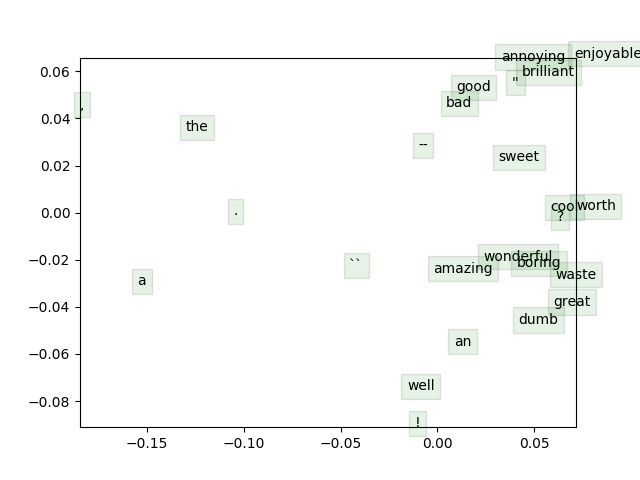
\includegraphics[scale=1.0]{q3_word_vectors.png}
	\label{figure:wordvectors}
	\caption{Word Vectors}
\end{figure}


%----------------------
\subproblem{h}{CBOW (Extra Credit: 2 pts)}

\noindent \textbf{Answer:}  See code: $\sim$\verb|/q3_sgd.py|. \\




\newpage
%-------------------------------------
\problem{4: Sentiment Analysis (20 pts)}
%-------------------------------------

%----------------------
\subproblem{a}{Sentence Features (2 pts)}

\noindent \textbf{Answer:}  See code: $\sim$\verb|/q4_sentiment.py|.

%----------------------
\subproblem{b}{Purpose of Regularization (1 pt)}
\noindent \textbf{Answer:} \\

\noindent Purpose of regularization to constrain parameters, to avoid overfit on training dataset. And this can increase the generalizability of the model for new data.


\vskip5em



%----------------------
\subproblem{c}{Purpose of Regularization (1 pt)}
\noindent \textbf{Answer:}  See code: $\sim$\verb|/q4_sentiment.py|. \\

\textit {The chooseBestModel code}

\lstinputlisting[firstline=93, lastline=99]{q4_sentiment.py}

\vskip5em



\newpage
%----------------------
\subproblem{d}{Pretrained vs New Vectors (3 pts)}

\noindent \textbf{Answer:} \\

\textit{The Best train, dev and test accuracies using "Your Vectors" are around $31.2\%, 30.7\%, 29.6\%$ }
\begin{table}[!htbp]
\centering
\caption{Sentiment Accuracy with different Regularization rate-- "Your Vectors" - on Stanford Sentiment Treebank dataset}
\label{tab:yourvectors_sentiment}
\begin{tabular}{@{}r|lll@{}}
\toprule
\textbf{Regularization Rate $\lambda$} & \multicolumn{3}{c}{\textbf{Accuracy}}               \\ 
\textbf  { Use $\frac{1}{\lambda}$   }    & \textit{Train}  & \textit{Dev}    & \textit{Test}   \\ \midrule
0.000115                             & \textbf{31.262} & 30.699 & 29.593 \\
0.007920                           & 31.203         & \textbf{31.153} & \textbf{29.819}  \\
0.011000                               & 31.250          & 30.790           & 29.593          \\
0.107000                               & 30.466          & 30.881         & 29.276          \\
1.050000                               & 28.956          & 28.247          & 27.059          \\ \bottomrule
\end{tabular}
\end{table}

\textit{The Best train, dev and test accuracies using "Pretrained" are around $39.97\%, 36.6\%,37.3\%$ }
\begin{table}[!htbp]
\centering
\caption{Sentiment Accuracy with different Regularization rate -- Pretrained GloVe}
\label{tab:glove_sentiment}
\begin{tabular}{@{}r|lll@{}}
\toprule
\textbf{Regularization Rate$\lambda$} & \multicolumn{3}{c}{\textbf{Accuracy}}   		   \\ 
\textbf {Use $\frac{1}{\lambda}$}		& \textit{Train} & \textit{Dev}   & \textit{Test}  \\ \midrule
0.000115                              & 39.923        & 36.331		  & 37.014\\
0.000792                              & \textbf{39.970}& 36.240		  & 37.104         \\
0.011000                               & 39.899         & 36.240         & 37.195         \\
0.107000                               & 39.782         & \textbf{36.603} & 37.195         \\
1.050000                              & 39.478         & 36.512& \textbf{37.330}         \\ \bottomrule
\end{tabular}
\end{table}


\textit{ I think there below reasons making pretrained vectors did better \\
\begin{enumerate}
\item GloVe vector has higher dimensions ($D=50$) 
\item Wikipedia dataset (billion tokens), which GloVe (pretrained) using is much larger than SST (215 thousands phrases) 
\item GloVe use the global static information, while Word2Vec (skip-gram) not. 
\end{enumerate}
}
\vskip5em


\newpage
%----------------------
\subproblem{e}{Accuracy vs. Regularization (4 pts)}

\noindent \textbf{Answer:}\\

\begin{figure}[!htbp]\centering
	\label{figure:acc_vs_reg}
	\caption{Accuracy vs. Regularization}
	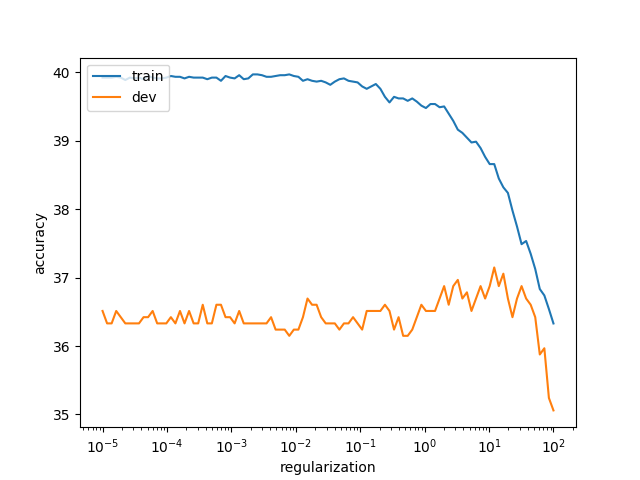
\includegraphics[scale=0.7]{q4_reg_v_acc.png}
\end{figure}
\noindent \textbf{Explain:}\\
\noindent In figure Accuracy vs. Regularization, the train accuracy and dev accuracy are better at $10^{-3}, 10^{-4}, and 10^{-5}$ regularization range, are around 40\% and 36.3\%. But the accuracy drops to 36\% and 35\% when regularization use $10^{1} and 10^{2}$. And also notice that the accuracy gap are around 4\% for regularization  $10^{-3}, 10^{-4}, and 10^{-5}$, which suggesting overfit on model, there is room to improve.

\newpage
%----------------------
\subproblem{f}{Confusion Matrix (4 pts)}

\textbf{Answer:}\\

\begin{figure}[!htbp]\centering
	\label{figure:confusionmatrix}
	\caption{Confusion Matrix (Development Set)}
	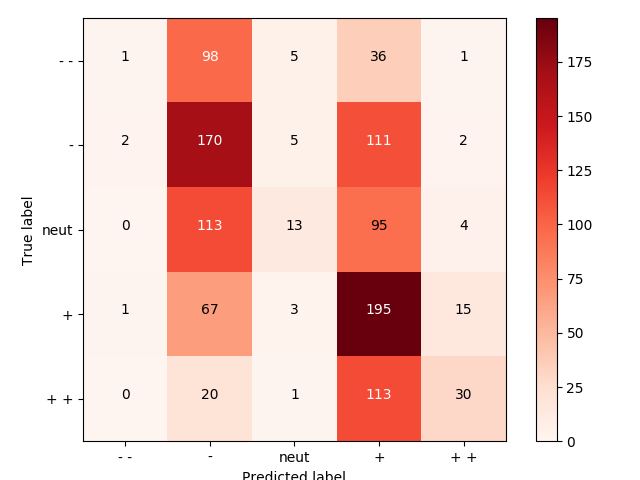
\includegraphics[scale=0.8]{q4_dev_conf.png}
\end{figure}
\noindent \textbf{Explain:}\\
\noindent  Interpret of the Confusion Matrix \\
The larger number in diagonal the better. We can see the model hard to tell "neutral" sentiment (value 13). And turn to put more "neutral" to "negative" (113 to 95). But model doesn't make huge mitake, like put "very negative" (--) to "very positive" (++) or vice versa.



\newpage 

%----------------------
\subproblem{g}{Error Types \& Features (4 pts)}
\noindent \textbf{Answer:} \\

\begin{enumerate}
	\item ``\verb|and if you 're not nearly moved to tears by a couple of scenes ,| \newline \verb|you 've got ice water in your veins .|''
	\subitem $\bullet$ True $= +$; Predicted $= -$
	\subitem $\bullet$ Model not understand the idiom  "moved to tears'', so not understand whole sentence
	%
	\item[] 
	%
	\item ``\verb|it 's slow -- very , very slow . .|''
	\subitem $\bullet$ True $= --$; Predicted $= netural$
	\subitem $\bullet$ Model need to have more context know this is a very positive sentence''.
	%
	\item[]
	%
	\item ``\verb|nothing is sacred in this gut-buster . .|''
	\subitem $\bullet$ True $= -$; Predicted $= +$
	\subitem $\bullet$ Say something in converse way. That's common error makes by word-based model.
\end{enumerate}


\end{document}
